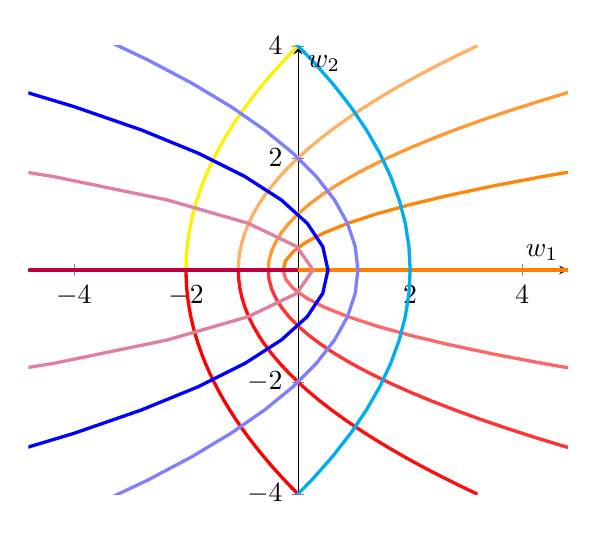
\begin{tikzpicture}
	\begin{axis}[
		axis lines=middle,
		axis equal,
		xmin=-4,
		xmax=4,
		ymin=-4,
		ymax=4,
		xlabel=$w_1$,
		ylabel=$w_2$,
	]
		
		\addplot[-, orange, very thick] coordinates {(0, 0) (5, 0)};
		
		\addplot[-, white!40!red, very thick, domain=-4:0] ({5/3*x^2 - 4/15},{x});
		\addplot[-, white!20!red, very thick, domain=-4:0] ({8/15*x^2 - 8/15},{x});
		\addplot[-, white!5!red, very thick, domain=-4:0] ({4/15*x^2 - 16/15},{x});
		\addplot[-, red, very thick, domain=-4:0] ({1/8*x^2 - 2},{x});
		
		\addplot[-, white!5!orange, very thick, domain=0:4] ({5/3*x^2 - 4/15},{x});
		\addplot[-, white!20!orange, very thick, domain=0:4] ({8/15*x^2 - 8/15},{x});
		\addplot[-, white!40!orange, very thick, domain=0:4] ({4/15*x^2 - 16/15},{x});
		\addplot[-, yellow, very thick, domain=0:4] ({1/8*x^2 - 2},{x});
		
		\addplot[-, purple, very thick] coordinates {(0, 0) (-5, 0)};
		
		\addplot[-, white!50!purple, very thick] ({-5/3*x^2 + 4/15},{x});
		\addplot[-, blue, very thick] ({-8/15*x^2 + 8/15},{x});
		\addplot[-, white!50!blue, very thick] ({-4/15*x^2 + 16/15},{x});
		\addplot[-, cyan, very thick] ({-1/8*x^2 + 2},{x});
	\end{axis}
\end{tikzpicture}